\documentclass[%
12pt,                % Schriftgröße
paper=a4,            % Papiergröße
captions=tableabove, % Beschriftungen für Tabellen oberhalb
]{scrartcl}

% ----------------------------------------------------
% Essential packages
% ----------------------------------------------------
\usepackage[utf8]{inputenc}
\usepackage[T1]{fontenc}

% ----------------------------------------------------
% Packages for layout adjustments
% ----------------------------------------------------

% Adjust line spacing
\usepackage{setspace}

% Publication quality tables
\usepackage{booktabs}

% ----------------------------------------------------
% Fonts
% ----------------------------------------------------
\usepackage{lmodern}
\renewcommand{\seriesdefault}{m}\selectfont

\newcommand\roboto{\fontfamily{Roboto-LF}\selectfont}
\newcommand*\robotocondensed{\roboto\fontseries{c}\selectfont}

\setkomafont{subject}{\large\robotocondensed}
\addtokomafont{title}{\LARGE}
\addtokomafont{subtitle}{\Large}
\setkomafont{author}{\normalsize\robotocondensed}
\addtokomafont{publishers}{\normalsize\robotocondensed}

% ----------------------------------------------------
% Colors
% ----------------------------------------------------
\usepackage{graphicx}
\usepackage[svgnames]{xcolor}
\definecolor{darkgreen}{rgb}{0.23,0.46,0.23}
\definecolor{smdsblue}{RGB}{0,69,134}

% ----------------------------------------------------
% Internal commands
% ----------------------------------------------------

\usepackage{etoolbox}
\makeatletter
\newcommand{\seminartype}[2]{%
  \subject{%
    Seminar\\
    \textit{\GetTranslationWarn{seminar@#1}}\\
    #2
  }
}
\newcommand{\advisor}[1]{%
  \publishers{%
    \GetTranslation{advisor}: #1\\
    \GetTranslation{institute}}
}
\newcommand{\email}[1]{\gdef\@email{#1}}
\newcommand{\matrno}[1]{\gdef\@matrno{#1}}
\newcommand{\institute}[1]{\gdef\@institute{#1}}
\makeatother

% Sprachauswahl:
%  main=* setzt die Hauptsprache für das Dokument
%  - ngerman --> deutsch
%  - english --> englisch
\def\languages{main=ngerman,english}
%\def\languages{main=english,ngerman}

% Art und Zeitpunkt des Seminars:
% - SEvS    Software Engineering für verteilte Systeme
% - AvioSE  Avionic Software Engineering
% - AutoSSE  Automotive Software and Systems Engineering
% - MIS     Medical Information Sciences
% - SEisS    Software Engineering in sicherheitskritischen Systemen
\seminartype{SEvS}{Sommersemester 2022}

% Haupttitel der Arbeit
\title{Key Challenges for Intent-Driven Mobile Network Management}
% Untertitel der Arbeit -- für Seminararbeiten nicht benötigt
% \subtitle{Concepts, Technologies, and Applications}

% Name, Matrikelnummer und E-Mail-Adresse
\author{Vladyslav Kolesnykov}
\matrno{2054429}
\email{vladyslav.kolesnykov@uni-a.de}

% Datum der Abgabe
\date{21.06.2022}

\advisor{Tobias Foth}

%%% Local Variables:
%%% mode: latex
%%% TeX-master: "Seminararbeit"
%%% End:


% ----------------------------------------------------
% Multi-lingual documents with Babel
% ----------------------------------------------------
\usepackage{csquotes}
\usepackage[\languages]{babel}

% ----------------------------------------------------
% Hyperlinks in PDF documents
% ----------------------------------------------------
\usepackage[%
bookmarks=true,         %
bookmarksopenlevel=1,   %
bookmarksopen=true,     %
bookmarksnumbered=true, %
plainpages=false,       % correct hyperlinks
pdfpagelabels=true,     % view TeX pagenumber in PDF reader
colorlinks=true,        % color highlight links
allcolors=black,        % make all links black by default
urlcolor=smdsblue,      % URL color
]{hyperref}

\makeatletter
\AtEndPreamble{
  \hypersetup{
    pdftitle=\@title,
    pdfauthor=\@author
  }
}
\makeatother

% Provides a solution to the problem with hyperref that links
% to floats actually anchor to the place below the float's caption,
% instead of anchoring to the beginning of the float
\usepackage[all]{hypcap}

% ----------------------------------------------------
% Code listings
% ----------------------------------------------------
\usepackage{listings}
\lstset{%
  frame=single,                             % Add a single line frame around listings
  frameround=ftft,                          % Rounded frame corners on top left and bottom right
  backgroundcolor=\color{gray!5},           % Slight gray shade for listings
  rulecolor=\color{black!30},               % Gray frame outline
  xleftmargin=.125\textwidth,               % Extra left margin
  xrightmargin=.125\textwidth,              % Extra right margin
  basicstyle=\small\ttfamily,               % General font style for listings
  keywordstyle=\bfseries,                   % Font style for keywords
  commentstyle=\color{gray},                % Font style for comments
  stringstyle={},                           % Font style for string literals
  numbers=left,                             % Show line numbers
  stepnumber=1,                             % Step increments for line numbers
  numberstyle={\sffamily\tiny\color{gray}}, % Font style for line numbers
  numbersep=2em,                            % Space between line numbers and code
}

% ----------------------------------------------------
% Bibliography management
% ----------------------------------------------------
\usepackage[%
backend=biber,      % Use biber to process bibliographies
natbib=true,        % Provide natbib-compatible citation commands
sorting=none,       % Sort citations by occurrence in the document
style=numeric-comp, % Use compressed numeric citations, e.g. [1-3; 5]
block=space,        % Add a little spacing inside bibliography entries
]{biblatex}
\addbibresource{literature.bib}

% Use main body font for URLs in bibliography
\urlstyle{same}

% Suppress page numbering on table of contents page(s). Works at least on one-page TOC.
\AtBeginDocument{\addtocontents{toc}{\protect\thispagestyle{empty}}} 

% Intelligent cross-referencing
% Note: Must be loaded at end of preamble (esp. after hyperref)
\usepackage{cleveref}

% ----------------------------------------------------
% Localization / translations
% ----------------------------------------------------
\usepackage{translations}

% Translations for seminar names
\NewTranslation{ngerman}{seminar@SEvS}{Software Engineering für verteilte Systeme}
\NewTranslationFallback{seminar@SEvS}{Software Engineering for Distributed Systems}
\NewTranslationFallback{seminar@AvioSE}{Avionic Software Engineering}
\NewTranslationFallback{seminar@AutoSSE}{Automotive Software and Systems Engineering}
\NewTranslationFallback{seminar@MIS}{Medical Information Sciences}
\NewTranslation{ngerman}{seminar@SEisS}{Software Engineering in sicherheitskritischen Systemen}
\NewTranslationFallback{seminar@SEisS}{Software Engineering in Safety- and Security-Critical Systems}

% Generic translation used in template
\NewTranslation{ngerman}{advisor}{Betreuer}
\NewTranslation{ngerman}{matrno}{Matrikelnummer}
\NewTranslation{ngerman}{institute}{Softwaremethodik für verteilte Systeme (Prof. Bauer)\\Universität Augsburg}
\NewTranslation{ngerman}{regularlit}{Literatur}
\NewTranslation{ngerman}{onlinelit}{Online-Quellen}
\NewTranslation{ngerman}{honesty@title}{Eidesstattliche Erklärung}
\NewTranslation{ngerman}{honesty@body}{%
  Ich versichere, dass ich die vorliegende Arbeit ohne fremde Hilfe und ohne Benutzung anderer
  als der angegebenen Quellen angefertigt habe, und dass die Arbeit in gleicher oder ähnlicher
  Form noch keiner anderen Prüfungsbehörde vorgelegen hat.\endgraf
  Alle Ausführungen der Arbeit, die wörtlich oder sinngemäß übernommen wurden, sind als solche
  gekennzeichnet.
}

% English fallback text
\NewTranslationFallback{advisor}{Advisor}
\NewTranslationFallback{matrno}{Matriculation number}
\NewTranslationFallback{institute}{Software Methodologies for Distributed Systems (Prof. Bauer)\\University of Augsburg}
\NewTranslationFallback{regularlit}{Literature}
\NewTranslationFallback{onlinelit}{Online resources}
\NewTranslationFallback{honesty@title}{Declaration of Academic Honesty}
\NewTranslationFallback{honesty@body}{%
  Hereby, I declare that I have composed the presented paper independently on my own and without
  any other resources than the ones indicated. All thoughts taken directly or indirectly from external
  sources are properly denoted as such.\endgraf
  This paper has neither been previously submitted to another authority nor has it been published yet.
}

%%% Local Variables:
%%% mode: latex
%%% TeX-master: "Seminararbeit"
%%% End:


\begin{document}
\pagenumbering{roman}	
\begin{titlepage}
  \onehalfspacing
  \makeatletter
  \vspace*{1em}
  \begin{center}
    \ifdefempty{\@subject}{}{%
      {\usekomafont{subject}\@subject}
      \par\vspace{2em}
    }
    {\usekomafont{title}\@title}
    \ifdefempty{\@subtitle}{}{%
      \par\vspace{.5em}
      {\usekomafont{subtitle}\@subtitle}
    }
    \par\vspace{2em}
    \singlespacing
    {\usekomafont{author}%
      \@author\par
      \GetTranslation{matrno}: \@matrno\par}
    \texttt{\@email}
    \par\vspace{1.5em}
    {\usekomafont{publishers}\@publishers}
  \end{center}
  \makeatother

  \begin{abstract}
    \noindent%
    \paragraph*{\abstractname}
    \textcolor{red}{Bitte Dateien \texttt{settings.tex} und \texttt{titlepage.tex} anpassen.}
    
    Lorem ipsum dolor sit amet, consectetuer adipiscing elit, sed diam nonummy nibh euismod tincidunt ut laoreet dolore magna aliquam erat volutpat. Ut wisi enim ad minim veniam, quis nostrud exerci tation ullamcorper suscipit lobortis nisl ut aliquip ex ea commodo consequat.
  \end{abstract}

  \vfill
  \centering
  
\includegraphics[height=38mm]{figures/uni_siegel}
\end{titlepage}
%%% Local Variables:
%%% mode: latex
%%% TeX-master: "Seminararbeit"
%%% End:


\tableofcontents

\clearpage
\pagenumbering{arabic}

\section{Introduction}
\label{sec:Introduction}
Intent-Driven Networking (IDN) is a promising network concept that has received great attention from industry and open source communities in recent years. Conventional networks are configured manually with specific execution commands. Instead, Intent-Driven Network is provided with desired business intent and does not require any exact configuration. This concept has the potential to automate the network management process by providing simple and powerful tools to handle resources, infrastructure, and services\cite{Mwanje2021}. However, there is no unified and clear definition of Intent-Driven Networking. The enabling techniques and frameworks of IDN are still in the further exploration phase\cite{8968429}.

\section{Basics}
\label{sec:Basics}

\subsection{Mobile Networks}
TODO: 5G and 6G Mobile Networks

\subsection{Software Defined Networking (SDN) / Network Functions Virtualization (NFV)}


\section{Intent-Driven Networking}
\label{sec:Intent_Driven_Networking}
The next section presents the formal definitions of Intent and Intent-Driven Networking. 

\subsection{Definition of Intent-Driven Networking}
Though different research institutions have proposed various definitions of intent and Intent-Driven Networking, all presented interpretations closely resemble each other. 

The intent can be described as a declarative way to define the desired state of the system that can be translated into an advanced policy. It abstracts the components and capabilities of the network from a requirements perspective. The intent does not define any specific commands on how to reach the resulting state. Instead, it only specifies the desired goal of the network\cite{Mwanje2021}. It means that the network should be able to understand the intent and map it into a specific device-level configurations.  The system automatically observes its current state and adjusts itself to achieve the desired outcome if there are any deviations. \cite[22867]{8968429}

Intent-Driven Networking (IDN) is a technology concept that tends to automate network administrative tasks by applying a deeper level of intelligence and intended state \cite{Kolibri}\cite{2022}. Intent-based networking captures, translates, and applies business intent across the network. The network is able to automatically deploy, configure, verify and optimize itself to achieve a target state defined by intent. The network performs continuous monitoring and adjustment to ensure alignment, which is achieved through a closed-loop system. Eventually, IDN provides full-lifecycle management for the network.\cite{8968429}

Intent-Driven Networking management provides four main functionalities: 

\begin{enumerate}
	\item Translation and verification. The IDN captures and translates business intent into the necessary system configuration, which is then automatically applied across the network. The system then validates the correctness of the resulting policy.
	\item Automatic deployment. The IDN installs translated and verified policies across physical and virtual network infrastructure through network automation and network orchestration.
	\item Network state awareness. The state of the network may constantly change, which can lead to some inconsistencies between implementation and the desired outcome. The system needs to continuously monitor and manage the network to guarantee fulfillment of the business intent at any point in time.
	\item Accurate diagnosis and dynamic optimization. The ultimate goal is for the network to continuously monitor and adjust network performance to ensure the desired business outcome. If expected intent is not achieved, the system takes corrective actions. \cite[271]{Wei2020}
\end{enumerate}









\subsection{Intent-Driven System Architecture}

\subsection{Closed-loop System}

\subsection{Intent Fulfilment}

\subsection{Advantages of Intent-Driven Networking}

\subsection{Challenges of Intent-Driven Networking}

\subsection{Industrial Products}

\section{Conclusion}
\label{sec:Conclusion}





\section{TODO: Delete}
\label{sec:Delete}
Abbildungen können z.\,B. im Unterverzeichnis \texttt{figures} abgelegt werden.
Eingebunden werden diese mit dem Befehl \texttt{\textbackslash includegraphics} innerhalb
einer \texttt{figure}-Umgebung:
\begin{figure}[htb]
  \centering
  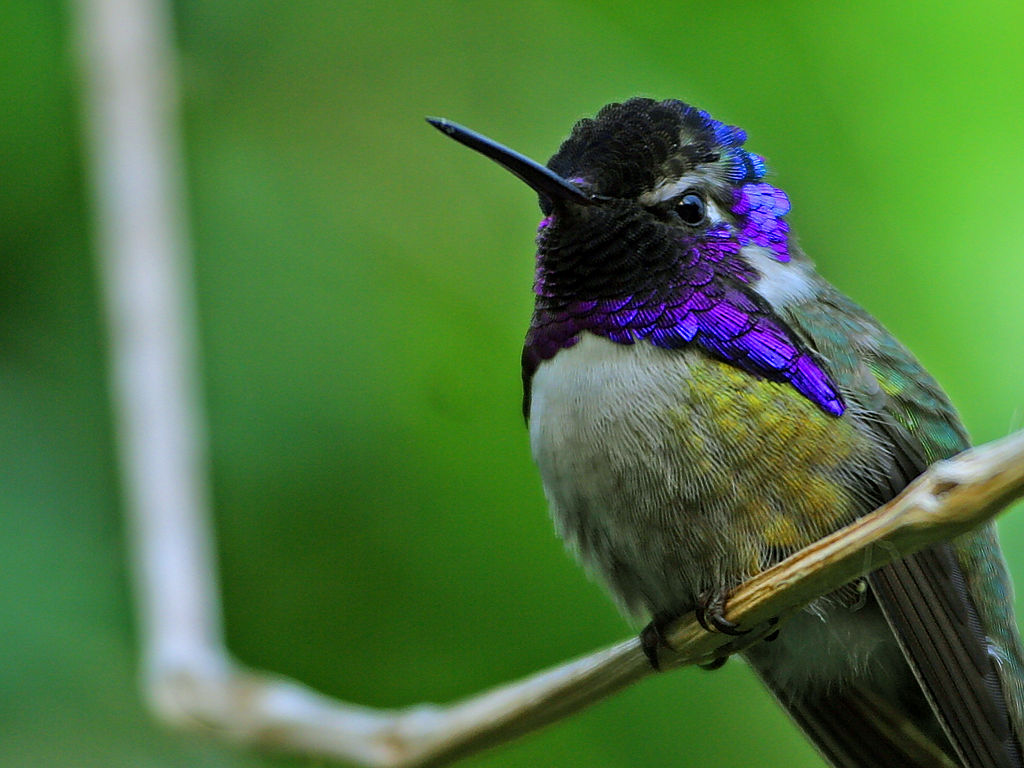
\includegraphics[width=0.8\textwidth]{figures/Hummingbird.jpg}
  \caption{Eine Veilchenkopfelfe (auch Costakolibri genannt, vom lateinischen Calypte costae), die zur Familie der Kolibris gehört \cite{Kolibri}}
  \label{fig:kolibri}
\end{figure}

\subsection{Erste Zwischenüberschrift}
\label{sec:ErsteZwischenueberschrift}
Die Arbeit kann auch Tabellen im \texttt{table}-Environment enthalten:
\begin{table}[ht]
  \centering
  \caption{Entfernungstabelle Süddeutschland, vgl. \cite{entfernungstabelle}}
  \begin{tabular}{c r r r}
    \toprule
              & Augsburg & München & Stuttgart \\
    \midrule
    Augsburg  & -        & 61      & 149       \\
    München   & 61       & -       & 210       \\
    Stuttgart & 149      & 210     & -         \\
    \bottomrule
  \end{tabular}
  \label{tab:entfernungen}
\end{table}

\subsubsection{Erste Unterüberschrift}
\label{sec:ErsteUnterueberschrift}

Das \texttt{listings}-Paket erlaubt es, Quellcode mit Syntax-Highlighting einzubinden:

\begin{lstlisting}[language=Python,float=ht,caption={Python-Programm zur Berechnung der Fakultätsfunktion},label=lst:factorial]
def fact(n):
    """Return the n-th factorial number"""
    if n == 0:
        return 1
    else:
        return n * fact(n-1)
  
# Test output
print fact(10)
print "Done"
\end{lstlisting}

In \Cref{lst:factorial} finden Sie eine rekursive Funktion zur Fakultätsberechnung.
  
\subsection{Zweite Zwischenüberschrift}
\label{sec:ZweiteZwischenueberschrift}

TEXT

% Literaturverzeichnis
\printbibliography[heading=bibintoc]

% Anhang
\include{appendix}

% Eidesstattliche Erklärung
\clearpage
\section*{\GetTranslation{honesty@title}}
\GetTranslation{honesty@body}

\vspace{2em}
\makeatletter
Augsburg, \@date
\par\vspace{1.5cm}
(\@author)
\makeatother

%%% Local Variables:
%%% mode: latex
%%% TeX-master: "Seminararbeit"
%%% End:


\end{document}